\documentclass[
11pt, % The default document font size, options: 10pt, 11pt, 12pt
codirector, % Uncomment to add a codirector to the title page
]{charter} 




% El títulos de la memoria, se usa en la carátula y se puede usar el cualquier lugar del documento con el comando \ttitle
\titulo{Detector automático de objetos para despensa inteligente} 

% Nombre del posgrado, se usa en la carátula y se puede usar el cualquier lugar del documento con el comando \degreename
\posgrado{Carrera de Especialización en Sistemas Embebidos} 
%\posgrado{Carrera de Especialización en Internet de las Cosas} 
%\posgrado{Carrera de Especialización en Intelegencia Artificial}
%\posgrado{Maestría en Sistemas Embebidos} 
%\posgrado{Maestría en Internet de las cosas}

% Tu nombre, se puede usar el cualquier lugar del documento con el comando \authorname
\autor{Ing. Santiago Andrés Bualó} 

% El nombre del director y co-director, se puede usar el cualquier lugar del documento con el comando \supname y \cosupname y \pertesupname y \pertecosupname
\director{Nombre del Director}
\pertenenciaDirector{pertenencia} 
% FIXME:NO IMPLEMENTADO EL CODIRECTOR ni su pertenencia
\codirector{John Doe} % para que aparezca en la portada se debe descomentar la opción codirector en el documentclass
\pertenenciaCoDirector{FIUBA}

% Nombre del cliente, quien va a aprobar los resultados del proyecto, se puede usar con el comando \clientename y \empclientename
\cliente{-}
\empresaCliente{-}

% Nombre y pertenencia de los jurados, se pueden usar el cualquier lugar del documento con el comando \jurunoname, \jurdosname y \jurtresname y \perteunoname, \pertedosname y \pertetresname.
\juradoUno{Nombre y Apellido (1)}
\pertenenciaJurUno{pertenencia (1)} 
\juradoDos{Nombre y Apellido (2)}
\pertenenciaJurDos{pertenencia (2)}
\juradoTres{Nombre y Apellido (3)}
\pertenenciaJurTres{pertenencia (3)}
 
\fechaINICIO{1 de septiembre de 2023}		%Fecha de inicio de la cursada de GdP \fechaInicioName
\fechaFINALPlan{1 de octubre de 2023} 	%Fecha de final de cursada de GdP
\fechaFINALTrabajo{15 de marzo de 2024}	%Fecha de defensa pública del trabajo final


\begin{document}

\maketitle
\thispagestyle{empty}
\pagebreak


\thispagestyle{empty}
{\setlength{\parskip}{0pt}
\tableofcontents{}
}
\pagebreak


\section*{Registros de cambios}
\label{sec:registro}


\begin{table}[ht]
\label{tab:registro}
\centering
\begin{tabularx}{\linewidth}{@{}|c|X|c|@{}}
\hline
\rowcolor[HTML]{C0C0C0} 
Revisión & \multicolumn{1}{c|}{\cellcolor[HTML]{C0C0C0}Detalles de los cambios realizados} & Fecha      \\ \hline
0      & Creación del documento                                 &\fechaInicioName \\ \hline
1      & Primera entrega                                  & 3 de Septiembre de 2023 \\ \hline
%1      & Se completa hasta el punto 4 inclusive                 & dd/mm/aaaa \\ \hline
%2      & Se completa hasta el punto 7 inclusive
%		  Se puede agregar algo más \newline
%		  En distintas líneas \newline
%		  Así                                                    & dd/mm/aaaa \\ \hline
%3      & Se completa hasta el punto 11 inclusive                & dd/mm/aaaa \\ \hline
%4      & Se completa el plan	                                 & dd/mm/aaaa \\ \hline
\end{tabularx}
\end{table}

\pagebreak



\section*{Acta de constitución del proyecto}
\label{sec:acta}

\begin{flushright}
Buenos Aires, \fechaInicioName
\end{flushright}

\vspace{2cm}

Por medio de la presente se acuerda con el Ing. \authorname\hspace{1px} que su Trabajo Final de la \degreename\hspace{1px} se titulará ``\ttitle'', consistirá esencialmente en la implementación de un prototipo de un sistema de alacena inteligente capaz de mantener un inventario de los objetos dentro de la misma, detectando los productos que ingresan y egresan en tiempo real, y tendrá un presupuesto preliminar estimado de \textcolor{red}{600} h de trabajo y \textcolor{red}{\$XXX}, con fecha de inicio \fechaInicioName\hspace{1px} y fecha de presentación pública \fechaFinalName.

Se adjunta a esta acta la planificación inicial.

\vfill

% Esta parte se construye sola con la información que hayan cargado en el preámbulo del documento y no debe modificarla
\begin{table}[ht]
\centering
\begin{tabular}{ccc}
\begin{tabular}[c]{@{}c@{}}Dr. Ing. Ariel Lutenberg \\ Director posgrado FIUBA\end{tabular} & \hspace{2cm} & \begin{tabular}[c]{@{}c@{}}\clientename \\ \empclientename \end{tabular} \vspace{2.5cm} \\ 
\multicolumn{3}{c}{\begin{tabular}[c]{@{}c@{}} \supname \\ Director del Trabajo Final\end{tabular}} \vspace{2.5cm} \\
%\begin{tabular}[c]{@{}c@{}}\jurunoname \\ Jurado del Trabajo Final\end{tabular}     &  & \begin{tabular}[c]{@{}c@{}}\jurdosname\\ Jurado del Trabajo Final\end{tabular}  \vspace{2.5cm}  \\
%\multicolumn{3}{c}{\begin{tabular}[c]{@{}c@{}} \jurtresname\\ Jurado del Trabajo Final\end{tabular}} \vspace{.5cm}                                                                     
\end{tabular}
\end{table}




\section{1. Descripción técnica-conceptual del proyecto a realizar}
\label{sec:descripcion}



El presente trabajo práctico busca implementar un sistema de alacena inteligente, el cual pueda mantener un inventario de los objetos dentro de la misma de forma autónoma y automática, mediante la detección de los productos que ingresan y/o egresan a la despensa en tiempo real, en el instante en que se agregan o se remueven.

Se ha observado que es una de las problemáticas mas frecuentes en el marco de las compras cotidianas para el hogar, es que las personas muestran una tendencia a olvidarse de las cosas que deben comprar. El objetivo principal de este proyecto es solventar esta problemática aplicando un método que la industria viene aplicando hace ya varios años: control de inventario. Ésto será realizado de forma automática mediante un conjunto de sensores capaces de detectar los objetos que ingresan o egresan a la despensa, de forma tal de poder llevar a cabo un conteo de los objetos presentes o faltantes, permitiendo tener siempre a mano el estado de la despensa (o alacena), lo que supondrá una mejora en la gestión de las cosas que se tienen en el hogar. También permitirá entender las necesidades de consumo diario, semanal, quincenal o mensual de los distintos productos presentes en el hogar, lo que facilitará la creación de listas de supermercado de forma periódica y automática. Además, se podrá consultar este estado desde cualquier lugar, mediante el acceso desde una aplicación. 

A día de hoy las grandes industrias están implementando mejoras y soluciones en los hogares de forma constante, tratando de modernizar todos los electrodomésticos, ambientes y elementos. Sin embargo, cuando nos paramos sobre nuestra problemática planteada,en las soluciones propuestas hasta la fecha, no existen soluciones que aborden esta problemática de forma clara, concisa y , por sobre todo, útil para la sociedad. En particular, hasta la fecha, lo más parecido a lo que se ha planteado, consta de una solución propuesta por Samsung: ha integrado a sus heladeras una aplicación que lleva un inventariado de la misma, pero de forma manual, siendo el usuario quien ingresa a mano qué objetos ingresa, y qué objetos utiliza o extrae.

Nuestra propuesta planea no solo superar con creces la oferta actual del mercado, buscando subsanar la problemática desde la raíz, sino que también tiene como objetivo el sentar precedentes para ser el principio de numerosos avances en cuanto a esta tecnología, la cual continúen mejorando la calidad de vida de las personas, impulsando un nuevo paradigma. 

Este nuevo paradigma, consiste en rediseñar las alacenas, incorporando tecnología del siglo XXI. El concepto de inventario ya está más que establecido en  industrias y empresas, las cuales se ven altamente beneficiadas en productividad gracias al ahorro de tiempo que esto conlleva entender no solo la distribución de los objetos, sino también cuando es necesario reponerlos. Ese mismo beneficio es el que vamos a estar trasladando a los hogares. Con esta nueva gestión de inventario en las alacenas, se pueden automatizar un sinfín de procesos y tomas de decisiones propias del hogar que quitan tiempo personal. Este inventario automático, va a permitir mejoras en los siguientes aspectos:

\begin{itemize}
    \item Entender los consumos del hogar de los distintos productos.
    \item Interpretar los tiempos de reposición de cada producto, lo que permite generar listas de compra para diferentes períodos.
    \item Conocer qué productos se tiene en tiempo real, permitiendo tomar decisiones sobre los menús para las siguientes comidas.
\end{itemize}

Para llevar a cabo este proyecto, se propone un módulo integral capaz de detectar el ingreso/egreso de los productos hacia la despensa, computar la cantidad de productos y mantener el inventario dentro de si mismo. Además, deberá tener la capacidad para comunicarse con la red, no solo para posibilitar detectar un mayor número de elementos, sino también para poder llevar a cabo un respaldo del inventario interno, de forma tal de poder disponibilizarlo al usuario desde otra interfaz (por ejemplo web o aplicación móvil). 
Todo va a estar orquestado por un núcleo de procesamiento (microcontrolador), el cual se comunicará con un lector de código de barras para detectar al producto. Luego, mediante llamados de API, se va a identificar al producto, y se va a proceder a realizar el cómputo para modificar el inventario.
El dispositivo deberá ser alimentado mediante una batería, ya sea desechable o recargable, de forma tal de independizar al usuario sobre la posición en la cual debe instalar al producto.
A continuación podemos ver en la figura \ref{fig:diagBloques} un diagrama de bloques sobre el prototipo:

\begin{figure}[htpb]
\centering 
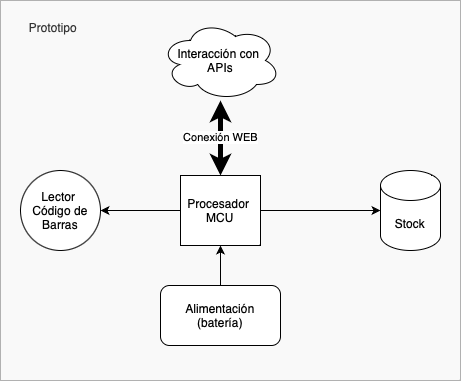
\includegraphics[width=.75\textwidth]{./Figuras/DiagramaBloque.png}
\caption{Diagrama en bloques del sistema propuesto.}
\label{fig:diagBloques}
\end{figure}

\vspace{25px}

\newpage

\section{2. Identificación y análisis de los interesados}
\label{sec:interesados}

A continuación se listan a todas las partes involucradas al proyecto:

\begin{table}[ht]
%\caption{Identificación de los interesados}
%\label{tab:interesados}
\begin{tabularx}{\linewidth}{@{}|l|X|X|l|@{}}
\hline
\rowcolor[HTML]{C0C0C0} 
Rol           & Nombre y Apellido & Organización 	& Puesto 	\\ \hline
Auspiciante   &           \authorname         &          -    	&        	\\ \hline
Responsable   & \authorname       & FIUBA        	& Alumno 	\\ \hline
Colaboradores &                   &              	&        	\\ \hline
Orientador    & \supname	      & \pertesupname 	& Director Trabajo final \\ \hline
Opositores    &                   &              	&        	\\ \hline
Usuario final &  Acreedores de alacena                 &              	&        	\\ \hline
\end{tabularx}
\end{table}


\begin{itemize}
	\item Auspiciante: siendo un proyecto personal, todos los gastos y/o beneficios serán incurridos por el autor del proyecto.
	\item Responsable: \authorname, quien va a ser el responsable del proyecto, siendo el autor del mismo.
 	\item Usuario final: como el proyecto esta orientado como solución para los hogares, el usuario final serán todas aquellas personas dueñas de una alacena.
 
\end{itemize}



\section{3. Propósito del proyecto}
\label{sec:proposito}

El propósito de este proyecto es impulsar nuevas tecnologías dentro del hogar mediante la modernización de uno de los lugares que más se utiliza dentro del mismo, posibilitando una mejor gestión de los distintos productos que se guardan dentro. Gracias a esta nueva metodología se busca que los usuarios encuentren una nueva forma mucho más sencilla y eficiente de la toma de decisiones en las compras cotidianas.

\section{4. Alcance del proyecto}
\label{sec:alcance}

En el proyecto se incluye :

\begin{itemize}
	\item El desarrollo de un dispositivo que detecta los objetos a través de una lectura del código de barras.
	\item Es desarrollo del dispositivo debe tener la capacidad para detectar de qué objeto se trata, y luego llevar a cabo el conteo relacionadas al inventario.
 	\item El desarrollo de una interfaz externa al dispositivo que permita consultar el estado del inventario.
  \item La misma interfaz debe tener la capacidad para configurar el dispositivo.
  \item El desarrollo de una placa integrada como prototipo.
  \item La configuración de red para que el dispositivo pueda utilizar APIs para consultar el código de barras.
  \item El sistema de alimentación propio del prototipo.
  
\end{itemize}

No serán parte del proyecto los siguientes:

\begin{itemize}
	\item No se desarrollará un producto final para ser comercializado.
	\item No se contemplará almacenamiento externo o almacenamiento en la nube.
  
\end{itemize}

\section{5. Supuestos del proyecto}
\label{sec:supuestos}


Para el desarrollo del presente proyecto se supone que:

\begin{itemize}
	\item El dinero disponible será suficiente para la adquisición de los materiales requeridos.
	\item Se presume que todos los componentes originales con los que es planteado el proyecto tendrán stock.
 \item Todos los componentes se consiguen de forma local sin ningún impedimento.
  
\end{itemize}

\newpage

\section{6. Requerimientos}
\label{sec:requerimientos}


A continuación se enumerarán los requerimientos del proyecto:

\begin{enumerate}
	\item Requerimientos generales del sistema
		\begin{enumerate}
			\item El sistema debe detectar cuando se ingresa o se egresa un objeto de la despensa.
			\item El sistema debe tener la capacidad de identificar de qué objeto se trata.
			\item El sistema debe llevar a cabo un conteo de los objetos que ingresan y/o egresan.
    \item El sistema debe almacenar el inventario de forma local.
    \item El sistema debe tener una aplicación web/móvil para poder consultar el inventario en tiempo real.
           
		\end{enumerate}
	\item Requerimientos de Hardware
		\begin{enumerate}
			 \item El módulo deberá alimentarse a través de una batería.
			\item El módulo deberá poder comunicarse utilizando el Estándar IEEE 802.11 b/g/n
(WiFi).
            \item El módulo deberá poder comunicarse utilizando Bluetooth Low Energy (BLE).
            \item El módulo utilizará un único chip que integre el microprocesador y la conectividad WiFi/Bluetooth.
            \item El módulo deberá comunicarse vía API a la red para identificar el producto.
            \item El módulo deberá detectar los códigos de barras mediante un lector apropiado o cámara fotográfica.
		\end{enumerate}
	\item Requerimiento de firmware
         \begin{enumerate}
            \item El firmware del módulo deberá ser programado en lenguaje C.
            \item Se realizarán tests de forma independiente para cada módulo, y de integración para cada una de las funcionalidades del mismo.
            \item El firmware deberá priorizar el ahorro energético. 
         \end{enumerate}
	\item Requerimientos de Gestión
        \begin{enumerate}
            \item Se utilizará un repositorio público en Github como sistema de control de versiones.
         \end{enumerate}
	
\end{enumerate}

\section{7. Historias de usuarios (\textit{Product backlog})}
\label{sec:backlog}

En esta sección se enuncian las historias de usuario, asignándoles a cada una un puntaje según los siguientes aspectos:
    \begin{enumerate}
        \item Dificultad de la tarea/trabajo.
        \item Complejidad del trabajo.
        \item Riesgo asociado.
    \end{enumerate}

Para asignarles la ponderación, se utilizará una escala siguiendo la serie de Fibonacci, para lo cual un número mayor implica un mayor costo. Para calcular el Story Point, se sumarán las tres ponderaciones asignadas, y en caso de que el resultado no pertenezca a la serie, se le asignará el número superior más cercano.

\begin{enumerate}
    \item Como usuario quiero instalar el producto de forma sencilla.
        \begin{itemize}
            \item Dificultad: 5
            \item Complejidad: 5
            \item Riesgo: 8
            \item Story Point: 21
        \end{itemize}

     \item Como usuario no quiero estar pendiente de cambiar/recargar la batería.
        \begin{itemize}
            \item Dificultad: 13
            \item Complejidad: 13
            \item Riesgo: 3
            \item Story Point: 34
        \end{itemize}

    \item Como usuario quiero una interfaz de usuario sencilla.
        \begin{itemize}
            \item Dificultad: 2
            \item Complejidad: 3
            \item Riesgo: 5
            \item Story Point: 13
        \end{itemize}

    \item Como usuario quiero consultar mi inventario en todo momento.
        \begin{itemize}
            \item Dificultad: 3
            \item Complejidad: 8
            \item Riesgo: 2
            \item Story Point: 13
        \end{itemize}
    \item Como usuario quiero que el producto sea lo más pequeño posible.
        \begin{itemize}
            \item Dificultad: 13
            \item Complejidad: 8
            \item Riesgo: 5
            \item Story Point: 34
        \end{itemize}
\end{enumerate}

\section{8. Entregables principales del proyecto}
\label{sec:entregables}


Los entregables del proyecto son:

\begin{itemize}
	\item Diagrama de circuitos esquemáticos
	\item Código fuente del programa.
	\item Guía de usuario.
	\item Diagrama PCB.
	\item Archivos de fabricación.
\end{itemize}


\section{9. Desglose del trabajo en tareas}
\label{sec:wbs}

A continuación se listan las tareas, junto con su duración es (en horas de trabajo):

\begin{enumerate}
\item Planificación y gestión del proyecto (80 hs):
	\begin{enumerate}
	\item Realizar un plan de trabajo (10 hs)
	\item Determinar componentes (10 hs)
    \item Planificar la programación del firmware (20 hs)
	\item Redactar informes y presentaciones (30 hs)
    \item Redactar guía de usuario y otros documentos afines (10 hs)
	\end{enumerate}
\item Investigación previa (125 hs)
	\begin{enumerate}
	\item Investigar soluciones propuestas similares (20 hs)
	\item Investigar microcontroladores (10 hs)
	\item Investigar componentes periféricos afines (20 hs)
    \item Investigar el estándar de código de barras (10 hs)
    \item Investigar métodos de lectura de códigos de barra (30 hs)
    \item Investigar librerías y APIs afines (15 hs)
    \item Investigar protocolos WiFi y BLE (20 hs)
	\end{enumerate}
\item Desarrollo de Software (130 hs)
	\begin{enumerate}
	\item Desarrollo de drivers específicos para cada periférico (25 hs)
	\item Integración de drivers y librerías (15 hs)
	\item Elaborar máquina de estados para el flujo del programa (10 hs)
	\item Desarrollo de interfaz de usuario (30 hs)
    \item Implementación de FreeRTOS y Low Power Consumption (30 hs)
    \item Optimización del código (20 hs)
	\end{enumerate}
 \item Desarrollo de Hardware (145 hs)
	\begin{enumerate}
	\item Elección del microcontrolador (5 hs)
	\item Elección del sensor de código de barras (5 hs)
    \item Elección de integrados para los módulos WiFi y BLE (10 hs)
	\item Ensamblado de prototipo funcional (5 hs)
	\item Diseño del circuito electrónico final (30 hs)
    \item Diseño del PCB final (30 hs)
    \item Generar archivos de fabricación (40 hs)
    \item Optimización (20 hs)
	\end{enumerate}
 \item Fabricación de prototipo (60 hs)
	\begin{enumerate}
	\item Fabricado de la placa (10 hs)
	\item Compra de componentes (5 hs)
	\item Ensamblado de componentes (15 hs)
	\item Diseño y fabricación de la caja (30 hs)
	\end{enumerate}
  \item Pruebas, ensayos y validaciones (70 hs)
	\begin{enumerate}
	\item Ensayos de señales eléctricas (10 hs)
	\item Pruebas de comunicaciones WiFi y BLE (10 hs)
	\item Pruebas generales de integración (20 hs)
	\end{enumerate}
\end{enumerate}

Cantidad total de horas: (610 h)

\section{10. Diagrama de Activity On Node}
\label{sec:AoN}

\begin{consigna}{red}
Armar el AoN a partir del WBS definido en la etapa anterior. 

%La figura \ref{fig:AoN} fue elaborada con el paquete latex tikz y pueden consultar la siguiente referencia \textit{online}:

%\url{https://www.overleaf.com/learn/latex/LaTeX_Graphics_using_TikZ:_A_Tutorial_for_Beginners_(Part_3)\%E2\%80\%94Creating_Flowcharts}

\end{consigna}

\begin{figure}[htpb]
\centering 
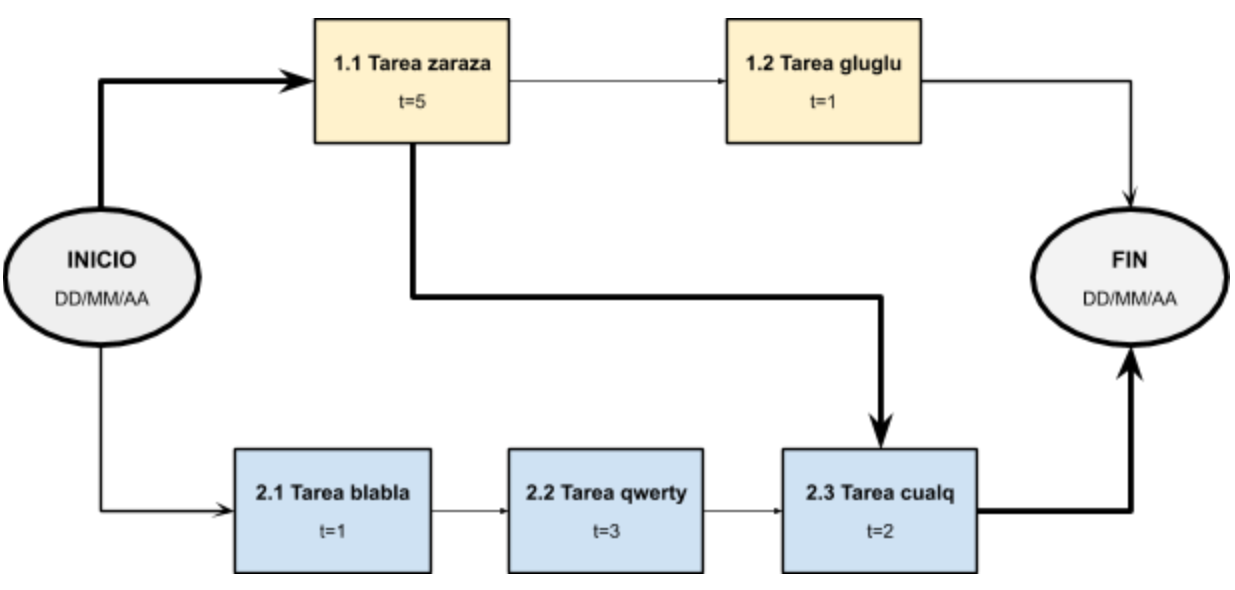
\includegraphics[width=.8\textwidth]{./Figuras/AoN.png}
\caption{Diagrama de \textit{Activity on Node}.}
\label{fig:AoN}
\end{figure}

Indicar claramente en qué unidades están expresados los tiempos.
De ser necesario indicar los caminos semicríticos y analizar sus tiempos mediante un cuadro.
Es recomendable usar colores y un cuadro indicativo describiendo qué representa cada color, como se muestra en el siguiente ejemplo:



\section{11. Diagrama de Gantt}
\label{sec:gantt}

\begin{consigna}{red}

Existen muchos programas y recursos \textit{online} para hacer diagramas de Gantt, entre los cuales destacamos:

\begin{itemize}
\item Planner
\item GanttProject
\item Trello + \textit{plugins}. En el siguiente link hay un tutorial oficial: \\ \url{https://blog.trello.com/es/diagrama-de-gantt-de-un-proyecto}
\item Creately, herramienta online colaborativa. \\\url{https://creately.com/diagram/example/ieb3p3ml/LaTeX}
\item Se puede hacer en latex con el paquete \textit{pgfgantt}\\ \url{http://ctan.dcc.uchile.cl/graphics/pgf/contrib/pgfgantt/pgfgantt.pdf}
\end{itemize}

Pegar acá una captura de pantalla del diagrama de Gantt, cuidando que la letra sea suficientemente grande como para ser legible. 
Si el diagrama queda demasiado ancho, se puede pegar primero la ``tabla'' del Gantt y luego pegar la parte del diagrama de barras del diagrama de Gantt.

Configurar el software para que en la parte de la tabla muestre los códigos del EDT (WBS).\\
Configurar el software para que al lado de cada barra muestre el nombre de cada tarea.\\
Revisar que la fecha de finalización coincida con lo indicado en el Acta Constitutiva.

En la figura \ref{fig:gantt}, se muestra un ejemplo de diagrama de Gantt realizado con el paquete de \textit{pgfgantt}. En la plantilla pueden ver el código que lo genera y usarlo de base para construir el propio.

\begin{figure}[htbp]
\begin{center}
\begin{ganttchart}{1}{12}
  \gantttitle{2020}{12} \\
  \gantttitlelist{1,...,12}{1} \\
  \ganttgroup{Group 1}{1}{7} \\
  \ganttbar{Task 1}{1}{2} \\
  \ganttlinkedbar{Task 2}{3}{7} \ganttnewline
  \ganttmilestone{Milestone o hito}{7} \ganttnewline
  \ganttbar{Final Task}{8}{12}
  \ganttlink{elem2}{elem3}
  \ganttlink{elem3}{elem4}
\end{ganttchart}
\end{center}
\caption{Diagrama de Gantt de ejemplo}
\label{fig:gantt}
\end{figure}


\begin{landscape}
\begin{figure}[htpb]
\centering 
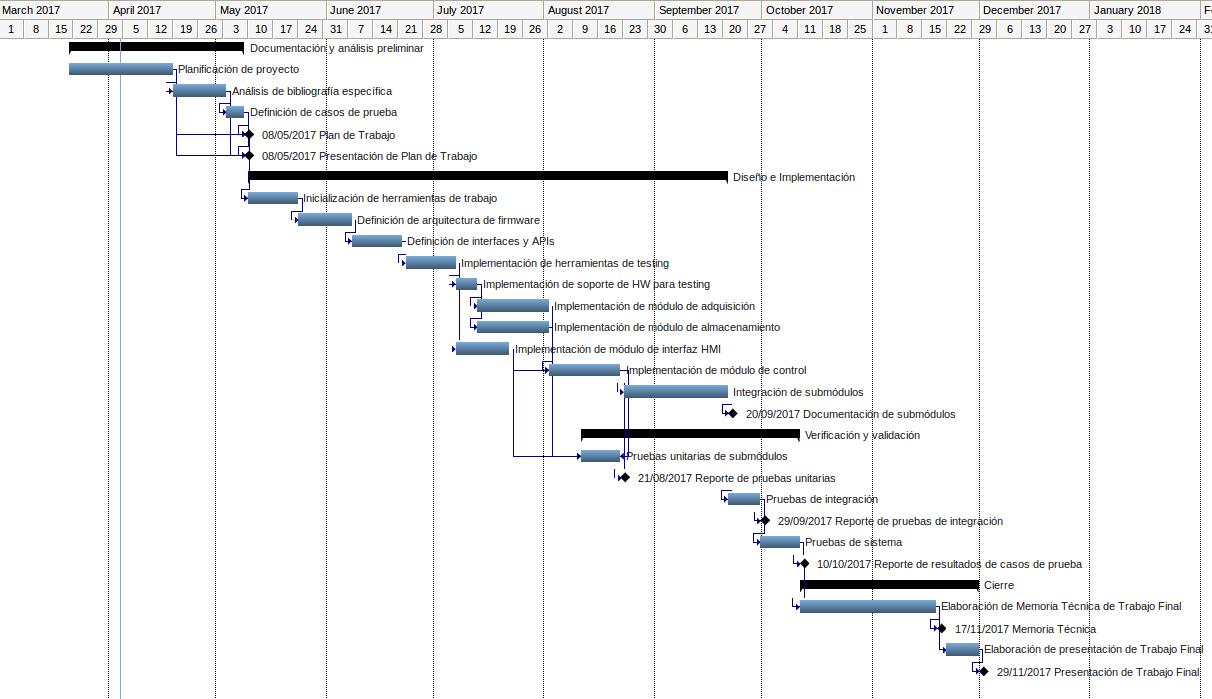
\includegraphics[height=.85\textheight]{./Figuras/Gantt-2.png}
\caption{Ejemplo de diagrama de Gantt rotado}
\label{fig:diagGantt}
\end{figure}

\end{landscape}

\end{consigna}


\section{12. Presupuesto detallado del proyecto}
\label{sec:presupuesto}

\begin{consigna}{red}
Si el proyecto es complejo entonces separarlo en partes:
\begin{itemize}
	\item Un total global, indicando el subtotal acumulado por cada una de las áreas.
	\item El desglose detallado del subtotal de cada una de las áreas.
\end{itemize}

IMPORTANTE: No olvidarse de considerar los COSTOS INDIRECTOS.

\end{consigna}

\begin{table}[htpb]
\centering
\begin{tabularx}{\linewidth}{@{}|X|c|r|r|@{}}
\hline
\rowcolor[HTML]{C0C0C0} 
\multicolumn{4}{|c|}{\cellcolor[HTML]{C0C0C0}COSTOS DIRECTOS} \\ \hline
\rowcolor[HTML]{C0C0C0} 
Descripción &
  \multicolumn{1}{c|}{\cellcolor[HTML]{C0C0C0}Cantidad} &
  \multicolumn{1}{c|}{\cellcolor[HTML]{C0C0C0}Valor unitario} &
  \multicolumn{1}{c|}{\cellcolor[HTML]{C0C0C0}Valor total} \\ \hline
 &
  \multicolumn{1}{c|}{} &
  \multicolumn{1}{c|}{} &
  \multicolumn{1}{c|}{} \\ \hline
 &
  \multicolumn{1}{c|}{} &
  \multicolumn{1}{c|}{} &
  \multicolumn{1}{c|}{} \\ \hline
\multicolumn{1}{|l|}{} &
   &
   &
   \\ \hline
\multicolumn{1}{|l|}{} &
   &
   &
   \\ \hline
\multicolumn{3}{|c|}{SUBTOTAL} &
  \multicolumn{1}{c|}{} \\ \hline
\rowcolor[HTML]{C0C0C0} 
\multicolumn{4}{|c|}{\cellcolor[HTML]{C0C0C0}COSTOS INDIRECTOS} \\ \hline
\rowcolor[HTML]{C0C0C0} 
Descripción &
  \multicolumn{1}{c|}{\cellcolor[HTML]{C0C0C0}Cantidad} &
  \multicolumn{1}{c|}{\cellcolor[HTML]{C0C0C0}Valor unitario} &
  \multicolumn{1}{c|}{\cellcolor[HTML]{C0C0C0}Valor total} \\ \hline
\multicolumn{1}{|l|}{} &
   &
   &
   \\ \hline
\multicolumn{1}{|l|}{} &
   &
   &
   \\ \hline
\multicolumn{1}{|l|}{} &
   &
   &
   \\ \hline
\multicolumn{3}{|c|}{SUBTOTAL} &
  \multicolumn{1}{c|}{} \\ \hline
\rowcolor[HTML]{C0C0C0}
\multicolumn{3}{|c|}{TOTAL} &
   \\ \hline
\end{tabularx}%
\end{table}


\section{13. Gestión de riesgos}
\label{sec:riesgos}

\begin{consigna}{red}
a) Identificación de los riesgos (al menos cinco) y estimación de sus consecuencias:
 
Riesgo 1: detallar el riesgo (riesgo es algo que si ocurre altera los planes previstos de forma negativa)
\begin{itemize}
	\item Severidad (S): mientras más severo, más alto es el número (usar números del 1 al 10).\\
	Justificar el motivo por el cual se asigna determinado número de severidad (S).
	\item Probabilidad de ocurrencia (O): mientras más probable, más alto es el número (usar del 1 al 10).\\
	Justificar el motivo por el cual se asigna determinado número de (O). 
\end{itemize}   

Riesgo 2:
\begin{itemize}
	\item Severidad (S): 
	\item Ocurrencia (O):
\end{itemize}

Riesgo 3:
\begin{itemize}
	\item Severidad (S): 
	\item Ocurrencia (O):
\end{itemize}


b) Tabla de gestión de riesgos:      (El RPN se calcula como RPN=SxO)

\begin{table}[htpb]
\centering
\begin{tabularx}{\linewidth}{@{}|X|c|c|c|c|c|c|@{}}
\hline
\rowcolor[HTML]{C0C0C0} 
Riesgo & S & O & RPN & S* & O* & RPN* \\ \hline
       &   &   &     &    &    &      \\ \hline
       &   &   &     &    &    &      \\ \hline
       &   &   &     &    &    &      \\ \hline
       &   &   &     &    &    &      \\ \hline
       &   &   &     &    &    &      \\ \hline
\end{tabularx}%
\end{table}

Criterio adoptado: 
Se tomarán medidas de mitigación en los riesgos cuyos números de RPN sean mayores a...

Nota: los valores marcados con (*) en la tabla corresponden luego de haber aplicado la mitigación.

c) Plan de mitigación de los riesgos que originalmente excedían el RPN máximo establecido:
 
Riesgo 1: plan de mitigación (si por el RPN fuera necesario elaborar un plan de mitigación).
  Nueva asignación de S y O, con su respectiva justificación:
  - Severidad (S): mientras más severo, más alto es el número (usar números del 1 al 10).
          Justificar el motivo por el cual se asigna determinado número de severidad (S).
  - Probabilidad de ocurrencia (O): mientras más probable, más alto es el número (usar del 1 al 10).
          Justificar el motivo por el cual se asigna determinado número de (O).

Riesgo 2: plan de mitigación (si por el RPN fuera necesario elaborar un plan de mitigación).
 
Riesgo 3: plan de mitigación (si por el RPN fuera necesario elaborar un plan de mitigación).

\end{consigna}


\section{14. Gestión de la calidad}
\label{sec:calidad}

\begin{consigna}{red}
Elija al menos diez requerientos que a su criterio sean los más importantes/críticos/que aportan más valor y para cada uno de ellos indique las acciones de verificación y validación que permitan asegurar su cumplimiento.

\begin{itemize} 
\item Req \#1: copiar acá el requerimiento.

\begin{itemize}
	\item Verificación para confirmar si se cumplió con lo requerido antes de mostrar el sistema al cliente. Detallar 
	\item Validación con el cliente para confirmar que está de acuerdo en que se cumplió con lo requerido. Detallar  
\end{itemize}

\end{itemize}

Tener en cuenta que en este contexto se pueden mencionar simulaciones, cálculos, revisión de hojas de datos, consulta con expertos, mediciones, etc.  Las acciones de verificación suelen considerar al entregable como ``caja blanca'', es decir se conoce en profundidad su funcionamiento interno.  En cambio, las acciones de validación suelen considerar al entregable como ``caja negra'', es decir, que no se conocen los detalles de su funcionamiento interno.

\end{consigna}

\section{15. Procesos de cierre}    
\label{sec:cierre}

\begin{consigna}{red}
Establecer las pautas de trabajo para realizar una reunión final de evaluación del proyecto, tal que contemple las siguientes actividades:

\begin{itemize}
	\item Pautas de trabajo que se seguirán para analizar si se respetó el Plan de Proyecto original:
	 - Indicar quién se ocupará de hacer esto y cuál será el procedimiento a aplicar. 
	\item Identificación de las técnicas y procedimientos útiles e inútiles que se emplearon, y los problemas que surgieron y cómo se solucionaron:
	 - Indicar quién se ocupará de hacer esto y cuál será el procedimiento para dejar registro.
	\item Indicar quién organizará el acto de agradecimiento a todos los interesados, y en especial al equipo de trabajo y colaboradores:
	  - Indicar esto y quién financiará los gastos correspondientes.
\end{itemize}

\end{consigna}


\end{document}
